\documentclass[11pt,letterpaper]{article}
\usepackage[pass]{geometry}
\usepackage{graphicx}
\usepackage{epsfig}
\usepackage{url}
\usepackage[english]{babel}
\usepackage{vmargin}
\usepackage{times}
\usepackage{amssymb}
\usepackage[fleqn]{amsmath}
\usepackage{cite}
\usepackage{titling}
\usepackage{color}

\usepackage{tikz}
\usetikzlibrary{positioning}
\definecolor{nodecolor}{RGB}{202,202,202}
\newlength\framesep
\setlength\framesep{16pt}
\pgfdeclarelayer{background}
\pgfsetlayers{background,main}
\pgfkeys{
	/tikz/node distance/.append code={
		\pgfkeyssetvalue{/tikz/node distance value}{#1}
	}
}

\widowpenalty=10000
\clubpenalty=10000


\begin{document}

\title{Total Platform Cyber Protection}
\date{}

\maketitle

\section{Introduction}

Traditional security defenses for the computing environment have
focused on securing the \emph{border} of the network, as this is the
entry place for most attackers. However, even with sophisticated
border technologies in place, there are constant attacks and data
breaches against our networks. The goal of this work is to survey the
state of security for the entire computing platform, in order to
identify specific areas that are underserved by the research community
and that require additional research and investment.

Modern computing infrastructure serves a wide array of needs, with
diverse technologies and implementations: embedded systems, cloud
computing, sensor networks, desktops, mobile devices, and industrial
control systems. Rather than consider each of these computing
platforms independently, in this work we abstracted the computing
platform into several layers, each of which are applicable to every
computing infrastructure. In particular, we analyzed the security
research performed at the following layers of the computing platform:
hardware, firmware, bus, hypervisor, operating system, application,
and network layers (Figure~1).

The goal of this work is to focus research effort on \emph{securing
  the entire computing platform.} An attack must effectively target a
specific vulnerability in a specific layer of the computing stack, and
an attacker uses that vulnerability to establish persistence on the
machine, potentially attacking the underlying computing layers of the
same machine or leveraging their place in the network to attack other
machines. Therefore, if we wish to increase the security of our
computing systems, and reduce the number and scope of security
breaches, it is essential that we encourage focus on novel ideas,
algorithms, and techniques to secure every level of the computing
stack.

In this report, we will first discuss the computing stack, and, for
every layer, we will describe the layer, identify primary threats
against the layer, and summarize the research on attempts to secure
that layer, and finally we will determine areas that require further
research investment to ensure the security of the layer.\begin{figure}
\centering
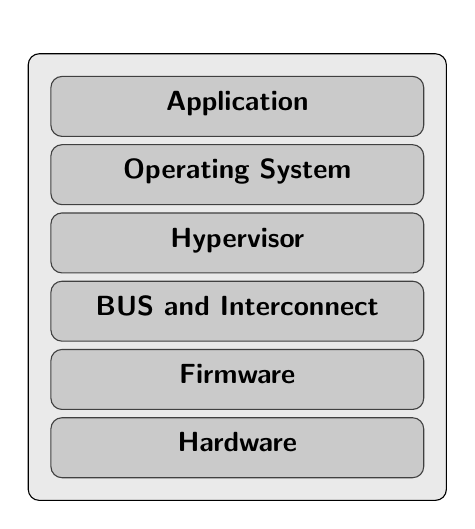
\begin{tikzpicture}[scale=0.50,node distance=3pt,outer sep=0pt,
platformlayer/.style={
  draw=darkgray,
  fill=nodecolor,
  rounded corners,
  text width=4.5cm,
  font={\sffamily\bfseries\color{black}},
  align=center,
  text height=9pt,
  text depth=6pt},
]
\node[platformlayer] (APP) {Application};
\node[platformlayer,below=of APP](OS) {Operating System};
\node[platformlayer,below=of OS] (HYP) {Hypervisor};
\node[platformlayer,below=of HYP](BUS){BUS and Interconnect};
\node[platformlayer,below=of BUS](FW) {Firmware};
\node[platformlayer,below=of FW](HW) {Hardware};

\begin{pgfonlayer}{background}
\draw[platformlayer,draw=black,fill=nodecolor!40]([xshift=-\framesep,yshift=1\framesep]current bounding box.north west)
rectangle ([xshift=\framesep,yshift=-\framesep]current bounding box.south east) 
node[below] at (0,2) {};

\end{pgfonlayer}
\end{tikzpicture}
\caption{Computing Platform Layers}
\label{fig:layers}
\end{figure}

\section{Background}

Here, we consider the diverse array of computing platforms as a number
of abstracted layers: hardware, firmware, bus, hypervisor, operating
system, application, and network layers. In this way, we can
categorize the research efforts that target each layer.

% Sai: should this be 'arranged' instead of 'arraigned'?%Faris: I think it should be 'arranged'.
The layers are arraigned from lowest to highest layer. The lower layer
has more control over the computing system, while the upper layers
have less control. For instance, the Hardware layer has total control
over the physical hardware and memory of the machine, while an
application running in the Application layer can only see a portion of
the machine's memory (because of the virtual memory used by the
Operating System).

A typical compromise, in relation to the proposed layers, is the
following: A vulnerability in an application is targeted, thus
allowing the attacker full control of the application layer. From
here, the attacker can scan the other applications on the network and
attempt to exploit those applications, thus spreading horizontally
throughout the network. Alternatively, as the application layer is the
least privileged and least persistent of the layers, the attack can
attempt to further the compromise on the lower layers of the machine.
For instance, the attacker can exploit the hypervisor layer to
compromise the host hypervisor. From this vantage point, the attacker
can transparently extract information from all the other guest
Operating Systems. More insidiously, the attacker can even exploit the
firmware level, which allows the attacker to persist even after
a complete reinstall of the operating system.

In our abstract model, the lower levels have more control over the
computing system, yet they have a smaller attacker surface. However,
the lower levels can be attacked by exploiting the upper levels. Also, the upper
levels trust the abstractions provided by the lower levels. For
instance, the application-layer visualization of an industrial control
system trusts that the data reported by the hardware layer is
accurate. If an attacker is able to control and manipulate the
hardware to falsely report the state of the system, the entire
integrity of the system can be compromised.

The interconnected nature of the layers means that the security of the
entire layer must be a priority. However, at the same time, the
security improvement of any layer will have an amplifying effect on
the security of the whole system. For instance, improvement to the
security of the application layer decreases the chance of an
application compromise, which further decreases the risk of the attack
propagating throughout the network and through the other layers.

\section{Hardware}

Hardware underpins all of modern computing. While most software is
constructed and written in such a way as to abstract the
peculiarities of the underlying hardware, the software cannot
execute without hardware. In our abstracted model of the computing
stack, hardware is at the bottom, which means that it has complete
control of the computing system.

For hardware here, we consider all types of hardware in the computing
system: CPUs, SoCs, or any other integrated circuit (IC) that performs
computation or communication on behalf of the upper computing layers.
This also includes networking cards and other peripheral devices
(Bluetooth or USB devices), which may have their own special purpose
embedded hardware.

A key difficulty in analyzing the security concerns of hardware is
reverse engineering the workings of the hardware. Traditional
techniques to reverse engineer hardware require destroying the chip,
and if a single hardware component is destroyed to reverse engineer,
there is no guarantee that other hardware is identical to the reverse
engineered chip.

\subsection{Threats}

As the lower-most level of the computing stack, all layers implicitly
trust that the hardware is executing correctly. Therefore, if an
adversary is able to maliciously control the hardware execution, they
can compromise all layers of the computing stack. Thus, the security
of the hardware is of paramount importance.

The main threat considered by the literature on hardware is the threat
of Trojan logic. This is malicious logic that is introduced into the
% adversary, by definition is a malicious entity.
hardware chip by an adversary. Trojan introduction can be
done at several points of the hardware lifecycle:

\begin{itemize}

\item \textbf{Design}. A malicious insider can incorporate a Trojan into the
  design of the hardware.

\item \textbf{Third-party IP}. Oftentimes, hardware designers will take
  advantage of the functionality of third-party components, using them
  as a black-box. Thus, a third-party can include malicious Trojan
  logic.

\item \textbf{Compilation of Design}. When the design of the hardware is
  compiled, but before it is sent for fabrication, the design could be
  changed to incorporate the Trojan logic. Note that this differs from
  Design-time, because the Trojan logic is not included in the design.
  Consider the case of malware on a hardware designer's machine, which
  changes the design when it is compiled.

\item \textbf{Manufacture}. A malicious manufacturer can introduce Trojan logic into hardware after the design is received but before the hardware
is fabricated.

\item \textbf{Delivery}. A malicious hardware component containing Trojan logic can be swapped with a benign component after fabrication but before
delivery and installation.
  
\end{itemize}

The malicious Trojan logic behavior comes in three different forms:
% Sai: is this three or two??

\begin{itemize}

\item \textbf{Trigger-based}. The malicious behavior or logic is only expressed when certain conditions are met. Consider a Trojan logic in a CPU,
  which changes the executing code to Ring 0 (with the most
  privileges) when a specific sequence of instructions are issued. The
  trigger can be internal to the chip, such as in the CPU case, or
  could be external, for instance a certain radio frequency will
  trigger the malicious code.

\item \textbf{Constant}. The malicious behavior or logic is continually
  executed and subtly changes the output of the hardware in a way that
  compromises security. Consider a Trojan logic of a Wi-Fi card, which
  leaks the Wi-Fi passphrase by embedding it in the operating
  parameters of the Wi-Fi radio.
  
\end{itemize}

These features of Trojan logic in hardware drive the research that
attempts to detect them. 

\subsection{Research}

Most research into hardware Trojans deal with using side-channel
analysis to identify the malicious Trojan behavior~\cite{Lee2005,
  Agrawal2007, Banga2008, Banga2008a, Jin2008, Du2010, Narasimhan2011,
  Narasimhan2012, Cao2013, Davoodi2013, Dworak2013, Forte2013,
  Liu2013, Liu2014, Bao2015}. This research uses power analysis, heat
analysis, or other side-effects to determine that the hardware is
executing abnormal logic. Unfortunately, this typically requires
building a model based on a ``golden'' or known-good hardware, which
is often not accessible. Furthermore, as chips become more complex,
the Trojan logic become an increasingly smaller portion of the chip,
which in turn reduces the side-channel behavior of the chip
significantly. 

Other research has demonstrated the attacks that are possible by
actually implementing Trojan behavior~\cite{King2008, Jin2010,
  Sturton2011, Liu2013, Jin2014, Zhang2014}. This line of research
shows that Trojan logic is feasible for an attack.

Of particular practical interest is a description of \emph{actual
  Trojan logic} discovered in the ProASIC3 Flash FPGA military
chip~\cite{Skorobogatov2012}. While in this case it was not proved
that the logic introduced to the chip was intentionally malicious,
nevertheless there existed functionality in the hardware that was
explicitly denied by the hardware designer. 

Another avenue of research is to change the design of the chip itself,
in order to improve the testability of the chip or to increase the
effectiveness of the side-channel analysis~\cite{Chakraborty2008,
  Li2008, Salmani2009, Hicks2010, Rosenfeld2011, Waksman2011,
  Bhunia2013, Davoodi2013, Rajendran2013, Rolt2014}. This line of
research attempts to rethink designing the hardware itself. However, a
major drawback is that this can increase the cost of the hardware and
it must be somehow mandated to be used in COTS components. 

JTAG is a main avenue of reverse engineering hardware, so some work
has investigated the problem of securing JTAG access to
hardware~\cite{Rosenfeld2010, Ren2015}. The main idea is to allow only
authenticated users to have access to the JTAG functionality, however
this increases the cost and complexity of implemented JTAG. 

Another approach is to change the design of the chip to support
runtime monitoring~\cite{Waksman2010}. In this way, the hardware
itself is monitoring itself, 
% Sai: can we rephrase this^ ? sounds weird %Faris : Removing the first 'itself' may solve the problem.
rather than external analysis of
side-channels. However, this has all the same drawbacks of changing
the design of hardware, in addition to not being robust in the face of
a powerful attacker who is able to alter the design. 

Recent approaches suggest to use machine-learning techniques to
identify the Trojan logic~\cite{Haider2015}. Another approach attempts
to use a formal verification technique in order to prove that no
malicious logic was added to the hardware~\cite{Guo2015}.

Finally, there are several surveys conducted on hardware security,
which provide a good overview of the field~\cite{Wang2008,
  Tehranipoor2010, Guin2014, Guin2014a, Guin2014b}.

Important problems include how to deal with counterfeit chips, better
non-destructive examination methods, continuous monitoring of the
integrity not just at boot time, and detection of backdoors and 
``undocumented features''.  Hardware design can also be done to
aid this process, e.g., having some part of the chip consume more power
to make it more identifiable for authentication purposes.  Other
possibilities include running multiple chips with different
implementations side-by-side and comparing results to detect unexpected
behavior.

\subsection{Suggested Focus Areas}

A key problem with hardware security is non-destructive IC
examination, identification, and authentication - how to ensure that
the chip that is designed is what is actually fabricated, with no
additional logic.

An additional neglected area is how to detect malicious Trojan logic
in third-party components. This would require some type of static
analysis or simulated dynamic analysis of third-party components,
which could detect Trojan logic.

Another approach that could be effective is how to properly test the
functionality of hardware after it has been fabricated. This could
include changing the design of the chip to allow better/more guided
fuzz testing of the chip itself, in order to discover the Trojan
logic.

Finally, a prevention approach could be taken, to monitoring the upper
layers of the computing stack for attempts to exploit the underlying
hardware. This can also include changing or altering the firmware
layer in such a way that it is not possible to exercise the Trojan
logic, potentially using randomization techniques similar to ASLR. 

\section{Firmware}

%Note: I did not remove the previous versions of those paragraphs
%(commented them) so feel free to check the previous versions and 
%revert them if my changes have problems.

%Firmware is the layer of software that sits and interacts directly
%with the hardware. Typically, the firmware is controlled from the
%upper layers by device drivers in the Operating System.

%Faris:
Firmware is the layer of software that sits and interacts directly
with the hardware. Typically, the firmware is controlled by the
device drivers in the upper layers of the Operating System.

%Many different hardware contain firmware, for instance the boot BIOS
%on a motherboard is a form of firmware, embedded systems often contain
%specific firmware, hardware peripherals such as network cards contain
%firmware as well. We consider all such areas as firmware.

%Faris:
Many different hardware contain firmware. For instance: the boot BIOS
on a motherboard, embedded systems that contain
specific firmware, hardware peripherals such as network cards. 
We consider all such areas as firmware.

%The key traits of firmware is that, although it is binary code, it is
%operating/interacting directly with the hardware, so there are no
%%OS-style abstraction layers such as virtual memory, well-defined
%system calls, or hardware abstraction. Therefore, each firmware is
%binary code which is specifically tailored to a specific hardware
%platform.

%Faris:
Although firmware is binary code, it is
operating/interacting directly with the hardware, so there are no
OS-style abstraction layers such as virtual memory, well-defined
system calls, or hardware abstraction which is the key trait of firmware. 
Therefore, each firmware is specifically tailored to a specific hardware platform.

%Due to the hardware-specific nature of firmware, \emph{reverse
%	engineering} is critical to understanding the firmware. In addition,
%reverse engineering is particularly challenging because source code is
%frequently unavailable, and vendors' desire to protect their
%intellectual property makes them actively obfuscate their
%firmware. All this means that, extracting semantically useful
%information from firmware is a key first step to performing any
%security analysis of the firmware.

%Faris:
Due to the hardware-specific nature of firmware, \emph{reverse
  engineering} is critical to understand it. In addition,
reverse engineering is particularly challenging because the source code is
frequently unavailable, and vendors' desire to protect their
intellectual property makes them actively obfuscate their
firmware. This means, extracting semantically useful
information from firmware is the first and key step to perform any
security analysis of the firmware.

\subsection{Threats}

As the lowest-level of software code in the computing stack, threats
to firmware can compromise the security of the entire machine.
Firmware security is concerned with two main threats: (1)
vulnerabilities in the firmware code itself which allow an attacker to
execute arbitrary code with the capabilities of the firmware and (2)
firmware with intentional Trojan (backdoor) capabilities.

%Vulnerabilities in the firmware code allow an attacker to execute
%arbitrary code with the permissions of the firmware. The class of
%vulnerabilities are not unique to firmware, as they are the same class
%of vulnerabilities that infect traditional binary software (buffer
%overflows, logic flaws, etc.). However, firmware typically has full
%control over the entire computing system, therefore vulnerabilities in
%firmware are much more severe than those in the application layer. In
%addition, if an attacker is able to persist their exploit --- because the
%compromise occurs at such a low layer of the computing system --- the
%attacker can persist \emph{even after reinstalling the operating
%	system or application}.

%Faris:
Vulnerabilities in the firmware code allow an attacker to execute
arbitrary code with the permissions of the firmware. The class of
vulnerabilities are not unique to firmware, as they are the same class
of vulnerabilities that infect traditional binary software (buffer
overflows, logic flaws, etc.). However, firmware typically has full
control over the entire computing system, therefore vulnerabilities in
firmware are much more severe than those in the application layer. In
addition, the attacker may remain in the system because the
compromise occurs at such a low layer of the computing system so the
exploit persists \emph{even after reinstalling the operating
system or application}.

%The attack surface for firmware varies depending on where it is used.
%In the most general case, the attacks can come from the upper layers,
%specifically the Operating System or Hypervisor layers, as these are
%the layers of the computing stack that can directly communicate with the
%firmware. However, other firmware can be attacked either directly
%through the Hardware layer itself, or through the data being
%transmitted through the firmware from the hardware. For instance, a
%network card firmware could be attacked through network traffic that
%the firmware processes.

%Faris:
The attack surface for firmware varies depending on where it is used.
In the general case, the attacks can come from the upper layers,
specifically the Operating System or Hypervisor layers, as these are
the layers of the computing stack that can directly communicate with the
firmware. However, other firmware can be attacked either directly
through the Hardware layer, or through the data being
transmitted through the firmware from the hardware. For instance, a
network card firmware could be attacked through network traffic that
the firmware processes.

Traditional vulnerability analysis is not effective on firmware, due
to the specificity of the firmware for the specific hardware and the
lack of a well-defined operating system abstraction for the firmware
code. In essence, each firmware is a custom binary with little in the
way of assumptions that vulnerability analysis can take advantage of. 

%Trojan capabilities in the firmware itself can allow a system to be
%remotely controlled or accessed. This is similar to a vulnerability,
%in that an attacker is able to control the firmware, however the key
%difference lies in the fact that Trojan behavior will be intentionally
%obfuscated by an attacker, whereas a vulnerability is accidentally
%introduced by a benign developer. Therefore, Trojan behavior is 
%more difficult to detect, because there is an active adversary who is
%intentionally obfuscating the behavior. 

%Faris:
Trojan capabilities in the firmware can allow a system to be
remotely controlled or accessed. This is similar to a vulnerability,
in that an attacker is able to control the firmware, however the key
difference lies in the fact that Trojan behavior can be intentionally
obfuscated by an attacker, whereas a vulnerability can accidentally
introduced by a benign developer. Therefore, Trojan behavior is 
difficult to detect.

%Vulnerabilities in the firmware and Trojan capabilities are related
%because both require \emph{understanding} the behavior and semantics
%of the firmware code. This is why reverse engineering is such a
%critical component of securing the threats against the firmware layer:
%in order to detect either vulnerabilities or Trojan functionality, an
%automated tool must first understand the semantics of the particular
%firmware/hardware combination. 

%Faris:
Vulnerabilities in the firmware and Trojan capabilities are related
because both require \emph{understanding} the behavior and semantics
of the firmware code. This is why reverse engineering is such a
critical component of securing the firmware layer against the threats.
In order to detect vulnerabilities or trojan functionality, an
automated tool must understand the semantics of the particular
firmware/hardware combination. 

\subsection{Research}
%Faris: Some fixes below. 
Researchers have attempted to identify real-world attacks on firmware
code~\cite{Tsow2006, Cui2010, Duflot2011, Basnight2013, Cui2013,
  Zaddach2013, Zaddach2013a, Maskiewicz2014, Stuttgen2015}. These
attacks are particularly effective, and researchers have shown that
these are able to persist through a reboot and cannot be detected by
the upper layers. 

Other approaches are about how to prevent the tampering of
firmware~\cite{Adelstein2002, Zhou2007, Zhou2009}. These protect from
the threat of tampering or altering the firmware, however it does not
address vulnerable firmware. 

Another approach includes runtime monitoring into the
firmware, so that compromises can be detected~\cite{Cui2010a,
  Cui2011}. This approach is further complicated by the lack of
abstractions in the firmware environment. 

Recent work has looked into the problem of updating the design of the
firmware so that it has security features, such as memory handling and
avoiding information leakage~\cite{Koeberl2014, Kauer2007}. However,
forcing firmware developers to use such features is an open issue.

Very few work has looked into how to reverse engineer and understand the
firmware~\cite{Zaddach2014}. This problem is of particular interest,
as understanding the semantics of the firmware and how it interacts
with hardware is a key challenge. 

Recent work has looked into how to detect vulnerabilities in
firmware~\cite{Davidson2013, Costin2014, Shoshitaishvili2015}. One of
these has an excellent website\footnote{\url{http://firmware.re}}
that contains the results of their reverse engineering and
vulnerability analysis~\cite{Costin2014}.

\subsection{Suggested Focus Areas}
%Faris: Some fixes below.
Of all the layers, firmware has received the least attention from the
research community. Therefore, we believe that focus on this research
area will yield significant dividends. 

The major challenge with preventing firmware vulnerabilities is how to decouple
firmware from the hardware, potentially using emulation of the
hardware, in order to aid the analysis of the firmware. 

In a similar vein, there is need for automated reverse engineering tools,
including analysis of memory layouts, code modules, even answering the
simple question of what is code in a firmware binary and what is data.

Finally, even if we find vulnerabilities or Trojan logic in a
firmware, there is still the unanswered question of how to patch or
update the functionality of the firmware while still guaranteeing the
behavior of the firmware. This is particularly complicated due to the
real-time requirements of the firmware and the potentially concurrent
executions.  

\section{Bus and Interconnect}

The Bus and Interconnect is an abstract layer of the computing system
which allows the firmware and hardware to communicate with each other.
Different computing architectures have different technical
implementations of the bus and interconnect. For instance, the
communication network in the automotive system, which has received
significant attention from the research community, uses a CAN bus to
communicate. Modern motherboards use either a Northbound or Southbound
bus --- such as USB --- to communicate between the CPU and other peripheral devices.

\subsection{Threats}

Depending on the technical architecture of the bus and interconnect
layer, the bus can be used either purely for communication or for
other functionality as well. For instance, the CAN bus is only used to
allow different hardware components to communicate. However, on modern
motherboards, techniques such as Direct Memory Access (DMA) allow a
peripheral device that is connected to the bus to directly access the
system's memory, without going through the CPU. 

In the case of the bus and interconnect being used as a communication
medium, then the classic threats are the same security concerns as
other mediums of communication: communication integrity and
confidentiality. A malicious device on the bus can impersonate another
device and send messages on the bus as the impersonated device. On an
automotive system, researchers have demonstrated that by compromising
a single device attached to the system's CAN bus allows an attacker to
have complete control over all functions of the automobile, by
impersonating messages on the CAN bus. In addition to impersonating
messages, an attacker on the bus and interconnect layer can listen to
messages on the bus, potentially eavesdropping on sensitive messages.

If the bus and interconnect layer offers advanced functionality, such
as the DMA example, then the devices that an attacker is able to connect
to the bus could take advantage of this functionality. In the case of
DMA, this means that any device on the bus has full access to the
physical memory of the system, therefore the attacker has complete
control over the upper layers of the computing system (hypervisor,
operating system, and application).

The difficulty of addressing the threats of the bus and interconnect
layer is the diversity and specificity of the specific bus and
interconnect technology. Often, these were created without
consideration for security needs, therefore, as a communication
mechanism they lack authentication from the design. In addition, as
the bus and interconnect layer cause different hardware to
communicate, all hardware must agree on the protocol to talk on the
bus. Therefore, adding security to the bus and interconnect protocol
is difficult in legacy systems.  

\subsection{Research}

A major area of research in the Bus and Interconnect layer is work
that shows the dangers of a bus and interconnect that allows malicious
devices to either impersonate devices on the bus or leverage bus
capabilities, particularly in the automotive area~\cite{Bonkoski2013,
  Checkoway2011, Hoppe2008, Koscher2010, Rouf2010, Sang2010}.

The other major area of research is to apply encryption to devices on
the bus and interconnect~\cite{Groza2012, Herrewege2011, Jiang2012,
  Schweppe2011, Stewin2014, Szilagyi2010}. In this way, malicious
devices on the bus cannot impersonate other devices. However, a key
problem with this research direction is how to distribute the keys of
the devices, which is typically done by distributing them in hardware.
Unfortunately, this approach is brittle, as it disallows new devices
from accessing the bus and interconnect.

Other research has investigated how to ensure the integrity of devices
attached to the bus and interconnect using attestation
techniques~\cite{Li2010, Li2011}. These techniques attempt to ensure
that only authorized and unmodified devices are attached to the bus
and interconnect. However, this research has the problem of how to
allow third-party devices to access the bus.

A key problem is how to perform secure updates to devices attached to
the bus and the interconnect~\cite{Larson2008}. This is a challenge
that also has similarities with the firmware layer.

In order to discover malicious communication, researchers have
utilized data flow tracking techniques to discover how the data flows
between devices connect to the bus and interconnect
layers~\cite{Schweppe2012}. Using these techniques, the researchers
are able to identify malicious flows or potential vulnerabilities by
analyzing the way that data flows throughout the system.

Other researchers have explored modeling either the system itself
or the behavior of the devices on the bus~\cite{Stewin2013a,
  Drolia2011}. If the device behavior or the system behavior does not
match the learned model, then an alert is triggered. In this way,
these techniques are similar to anomaly detection techniques, with
similar benefits and drawbacks. 

In order to address the issue of devices on the bus able to access
capabilities unauthorized, researchers have tackled the similar
problem of reducing the Trusted Computing Base, essentially reducing
the functionality of the bus and interconnect
layer~\cite{Vasudevan2012, Zhang2013, Zhou2009}. In this way, if the
functionality is not there on the bus, then a malicious device cannot
take advantage of it.

Another approach is to leverage hardware features of the underlying
bus and interconnect system to reduce the impact of an
attack~\cite{Wolf2012, Wojtczuk2011}. However, as these hardware
functionalities must be implemented, it's impact in legacy systems is
limited.

Finally, other research in this area has performed surveys of the
research on this area~\cite{Kleberger2011, Studnia2013, Thom2008,
  Wolf2004, Wolf2007, Wright2011, Zhao2002}.

\subsection{Suggested Focus Areas}

Further research in this area should focus on enabling better
monitoring of the runtime of devices attached to the bus or
interconnect. There is also the need to support logging of the bus or
interconnect activity. This will enable detection of a malicious
device on the bus or interconnect.

Another promising area of research is the automated filtering of
the bus communication, potentially allowing an administrator to define
a policy for a specific bus or interconnect system. This would be
particularly effective if it can be implemented on legacy bus and
interconnect systems, with no modification to the devices.

A different approach would be to secure the bus by only allowing
authorized devices to attach to the bus. This could be a white-listing
based approach or other policy-driven approach. However, the key
question is how to identify a device, particularly a third-party
device.

While there has been some research on encrypting the communication on
the bus, most has focused on pre-distributing the keys to devices on
the bus. This approach is brittle, as new devices cannot be added to
the bus easily. Therefore, further approaches should be investigated,
such as using attribute-based encryption to be able to encrypt and
distribute messages on the bus without prior sharing of keys.

\section{Hypervisor}

The purpose of the hypervisor layer is to provide virtualization
techniques for the upper layers of the computing stack. In essence,
the Hypervisor layer provides a virtualization or emulation of the
lower layers of the computing stack, so that multiple Operating
Systems, which each assume that they are the sole users of the
underlying hardware, can run concurrently on the same hardware.

For discussing the Hypervisor layer, we use the term \emph{host} to
define the hypervisor itself (which, in some cases can be an Operating
System) and the \emph{guest} is the Operating System that is running
on the hypervisor. A host can run multiple guest Operating Systems.

Hypervisors have a number of benefits, from allowing greater sharing
and usage of hardware resources, to improving the isolation of the
Operating Systems. The security benefits of using Hypervisors comes
from each guest Operating System being isolated from the other. In
theory, this means that a compromise of a guest Operating System will
be isolated to only that Operating System, and the attack should not
spread to other guest Operating Systems.

\subsection{Threats}

The central threat to the Hypervisor layer is from attackers in a
guest Operating System exploiting a vulnerability in the hypervisor
itself to gain access to the actual hardware or to propagate their
attack to the other guest Operating Systems that are running in the
hypervisor. As the Hypervisor layer is essentially emulating the
hardware for the guest operating systems, it has a large attack
surface. Furthermore, modern hypervisors, in an attempt to increase
the performance of the hypervisor, frequently allow guest Operating
Systems direct access to the hardware. If the hardware does not
provide for full isolation (i.e., it is not hypervisor-aware), then an
attacker can leverage this hardware to tamper or extract sensitive
information from other guest Operating Systems.

In modern hypervisors, the hypervisors frequently provide isolation
from a well-behaved guest Operating System, as the guest Operating
System is assumed to be benign. This assumption can be unfounded, as
the guest Operating System can be hostile and can attempt to exploit
or crash the hypervisor. 

Another threat actually stems from the Hypervisor itself being
untrusted. In the cloud computing environment, the guest Operating
System does not trust the underlying Hypervisor, as it is controlled
by a third-party. In this case, the Hypervisor can spy on the guest
or alter the memory of the guest.

\subsection{Research}

One area of research is to leverage the vantage point of the
Hypervisor to monitor the guest for security
violations~\cite{Karger1991, Barham2003}, intrusion
detections~\cite{Dunlap2002, Garfinkel2003a, Kourai2005, Chen2008,
  Garfinkel2003b}, checking the integrity of the guest Operating
system~\cite{Seshadri2006, McCune2010}, and identifying rootkits present
in the guest Operating System~\cite{Jones2008, Grace2010}. This work
assumes that the guest can be compromised and that the Hypervisor is
trusted, which, due to vulnerabilities in the Hypervisor, is not
always true.

A significant problem in monitoring or otherwise inspecting a guest
Operating System from the hypervisor layer is the \emph{semantic gap}
problem, where the Hypervisor has no outside knowledge of the
guest-specific Operating System constructs. Therefore, research has
investigated how to overcome this semantic gap~\cite{Jones2006,
  Christodorescu2009, Srinivasan2011}.

Further work in this line has approached the problem of how to monitor
the hypervisor itself by leveraging hardware features~\cite{Azab2010}.

In order to build a secure Hypervisor, the lower layers of the
computing system must also be trusted. Therefore, research into
establishing a Trusted Computing Base, which validates the integrity
of the lower levels for the guest Operating System~\cite{Arbaugh1997,
  Sailer2004, Singaravelu2006} is important for ensuring the security
of the Hypervisor.

One problem of using the Hypervisor as a security primitive is that it
is part of the Trusted Computing Base for the upper layers of the
computing platform. Therefore, attempts have been made to reduce the
trusted base of the Hypervisor itself~\cite{Murray2008, Shinagawa2009,
  Colp2011, Wang2012}.

Other research has looked at creating a secure
Hypervisor~\cite{Robin2000, Belay2012, Szefer2011, Vasudevan2013} with
the possibility of adding functionality to the Hypervisor to support
closed guest Operating Systems~\cite{Garfinkel2003}, offering
applications running in the guest Operating System to hide information
from the guest Operating System~\cite{Chen2008, Yang2008, Jin2011,
  Szefer2012, Azab2011, Zhang2011, Jin2011a, Szefer2011a}, secure
information flow between the guest Operating System drivers and I/O
devices~\cite{Cheng2013}, or designing the hypervisor so that it can
prove that it did not tamper with the guest Operating
System~\cite{Gu2011}.

Another approach to improve the security of the Hypervisor is to
remove the duplicated components from the guest Operating System
layer~\cite{Kivity2014, Madhavapeddy2015}, which effectively reduces
the attack surface of the Operating System layer.

Another interesting approach is to run traditional network middleware
boxes, such as firewalls and Intrusion Detection Systems, as a guest
Operating System of a Hypervisor~\cite{Martins2014}.

Finally, there have been attempts to introduce traditional
application-level security features to Hypervisors, in order to reduce
or prevent vulnerabilities, such as control-flow
integrity~\cite{Wang2010} or manual vulnerability
analysis~\cite{Perez-Botero2013}.

\subsection{Focus Areas}

As the hypervisor is typically a monolithic trusted entity, research
should be performed to reduce the trust in the hypervisor. One avenue
could be to have fine grained access control within the hypervisor, so
that different policies can be set to the guests hosted by the
hypervisor.

In a similar area, we believe that further research into reducing the
attack surface of the hypervisor is necessary. Specifically, the
hypervisor can be customized based on the applications and workload
necessary. 

Hypervisors, despite their obvious benefits, have not been applied to
real-time systems. Further research must be done to allow reliable and
robust hypervisors in a constrained real-time computing environment.

Testing hypervisors is currently a difficult and essentially manual
process. There is currently no equivalent to fuzz testing a hypervisor
implementation, possibly because there are no models for attacks
against a hypervisor. Further research in increasing the testability
and automated analysis of hypervisor reliability would improve security.

\section{Operating Systems}

The Operating System layer is responsible for ensuring that multiple
applications are able to concurrently run, without interfering with
each other. In addition, the Operating System layer is also
responsible for providing a unified abstraction of the underlying
hardware layer for the application layer. Therefore, in terms of
security, the Operating System layer has more privileges than the
application layer, as the Operating System controls the execution and
scheduling of processes, the access control policies that allow one
application to hide information/data from the other processes.

\subsection{Threats}

The main threat to the Operating System layer is an attacker
compromising the security of the Operating System. There are two main
avenues to how this compromise can occur: (1) an attacker exploits a
vulnerability in the Operating System from the Application layer or
(2) an attacker compromises a lower layer (for instance, modifying the
Operating System code directly to the hardware's Hard Drive).

Vulnerabilities in the Operating System allow an attacker to have
complete control over the other application running in the operating
system. In addition, the attacker can use their vantage point at the
operating system to attempt to escalate their attack to the hypervisor
or lower layers, such as the firmware. Vulnerabilities in the
Operating System result from programming errors that allow an attacker
to gain control of the Operating System code or data. These
vulnerabilities are traditional memory corruption vulnerabilities or
even logic flaws. 

A main concern in Operating System security is the presence of
rootkits, which are malicious modifications to the Operating System
which an attacker uses to achieve persistence on the system. In
addition, attackers use rootkits to hide from other applications on
the system. For instance, the rootkit will modify the operating system
code such that the attacker's processes and files are hidden from the
administrator or defensive software installed on the Operating System,
such as an anti-virus solution. 

Direct access to the hardware can allow an attacker to compromise the
Operating System. It is in this way that an attacker can propagate
their compromise from the lower layers of the computing platform to
the upper layers. The attacker has similar capabilities as when
exploiting a vulnerability in the Operating system.

\subsection{Research}

Research into Operating System security has a long and rich history,
which has looked at design flaws in Operating
Systems~\cite{Attanasio1973}. Further research looked at reducing the
permissions of the \emph{root} users, essentially compartmentalizing
the privilege of the Operating System~\cite{Kamp2000, Kurmus2014a}.

Rootkits attempt to persist the attacker's compromise of the operating
system and allow them to hide their malicious behavior from other
applications on the system. Therefore, rootkit detection is an
important research topic in Operating System
security~\cite{Petroni2004, Wang2005, Petroni2007, Payne2008,
  Sharif2009, Yin2010, Bianchi2012}. Another approach is to prevent
the rootkit from altering the Operating System
kernel~\cite{Riley2008a, Wang2009, Grace2010, Gadaleta2011}.

Vulnerability analysis techniques have been used to discover
vulnerabilities in the Operating System kernel before a hacker is able
to use and exploit those vulnerabilities. Static analysis techniques
have been used~\cite{Chou2001, Chen2011}.

Other vulnerability defenses include defenses for specific
vulnerability classes, such as buffer overflows~\cite{Dalton2008}.
Randomization techniques attempt to alter the environment of the
operating system in such a way that the system continues to function
but the attacker's exploit fails~\cite{Lin2009, Giuffrida2012}.
Control-flow integrity techniques have been applied to Operating
System code as well~\cite{Li2011a}.

Other research into Operating System security has looked at how to
protect applications from a malicious or compromised Operating
System~\cite{Ta-min2006, Onarlioglu2013, Li2014}.

% either driver code execute or change `and' to `is'
As driver code executes in kernel space, and is a frequent source of
vulnerabilities~\cite{Kadav2012}, researchers have looked into how to
make drivers more robust~\cite{Ganapathy2008, Hruby2012} or isolated
from the rest of the kernel~\cite{Boyd-Wickizer2010}.

Attack papers show that it is possible to compromise the kernel
without injecting any additional code, using Return Oriented
Programming techniques~\cite{Hund2009}.

A completely different approach is to formally prove the correctness
of the Operating System kernel~\cite{Klein2009}.

Updating Operating Systems with security updates is frequently
difficult, as the Operating System must be restarted. However,
researchers have explored how to apply an update to the Operating
System without rebooting the system~\cite{Arnold2009}.

Some work has been done on removing the operating system
entirely~\cite{Madhavapeddy2010} or trimming/tailoring parts of the
Operating System~\cite{Kurmus2011, Madhavapeddy2013, Howell2013,
  Kurmus2013, Kurmus2014}. This has the security benefit of reducing
the attack surface of the Operating System.

\subsection{Suggested Focus Areas}

We believe that, while significant research has been done on the
Operating System layer, there still remains work to be done in this
area. In particular, as the Operating System is frequently in contact
with malicious applications, it must be hardened from attack.

Therefore, we believe that further research into the line of trimming
or tailoring the operating system is important, such that the attack
surface is significantly reduced.

We also believe that non-control data-flow attacks will be the new
wave of attacks against Operating Systems. Therefore, we need new
analysis techniques, both static and dynamic, to discover these
vulnerabilities that do not require altering the control flow of the
Operating System.

A critical component of the Operating System is to handle the
execution of concurrent applications. Therefore, attacks that take
advantage of the concurrency in the Operating System are unexplored.
Research must be done to create new models for these attacks. 

\section{Application Layer}

The application layer is the layer of the computing stack that
performs that actual useful computation or offers the computing
service. It is essentially at the top of the computing stack, as the
lower layers of the computing stack provide abstractions so that
applications are easier to write and the upper layer (networking) is
used by the application layer to communicate to other applications.

At the application layer, we consider all the following types of
``applications'' under the application layer umbrella: GUI
applications, command-line applications, server batch process
applications, web applications, or mobile applications. Also, all
programming languages used to develop the applications are also in
scope, from compiled languages such as C or C++ to scripting languages
such as Python and Ruby. In short, all types of computing applications
are included in the application layer.

Due to abstractions provided by the lower layers, applications
typically have lesser privilege than the lower layers of the computing
stack. This is due to the abstractions provided to the application
layer, for instance an application cannot access the underlying hard
drive directly, but must use the Operating System's provided
interface.

Applications developed are typically very complex to understand
completely. This is due in part to the reliance on the abstractions
provided by the lower computing layers (as these abstractions must be
fully understood to understand how the application uses them). Another
aspect is that applications frequently use shared libraries or other
middleware, which are also considered to be part of the application
layer. In this way, multiple different applications can all use the
same underlying library. As the application's behavior depends on the
behavior of \emph{all} used libraries and abstractions, this means
that understanding even a simple application is dependent on the
complexity of the used abstractions.

\subsection{Threats}

Applications, by definition, must be accessible by users in
order to perform their useful computation. Due to this accessibility,
the application layer, of all the other computing layers, is the entry
point for attacks or exploits. 

At a high level the threat to the application layer is attackers being
able to influence the system to perform computation of their choosing.
There are two main vectors for an attacker to influence the system:
(1) software vulnerabilities in an application that can allow an
attacker to exploit the vulnerability to either perform arbitrary
computation or otherwise influence the application and (2) a malicious
application (typically described as a Trojan application) that the
attacker tricks the user into installing and running on the system,
usually by using social engineering techniques. 

Vulnerabilities are flaws or bugs in the application (or any software
for that matter) that allows an attacker to compromise the security of
the application. The key difference from normal flaws or bugs in
software is that vulnerabilities allow the program to deviate from the expected behavior. These vulnerabilities range the gamut of possible causes
such as programming errors or configuration mistakes. They can be in
the actual, custom application software or in any of the libraries
that the application uses. Some vulnerabilities are specific to a
given programming language, while others are more broad and can any
affect application. Examples of common vulnerabilities are: buffer
overflow, heap overflow, format string, off-by-one, integer overflow,
time-of-check-time-of-use, cross-site scripting, SQL injection, and
logic flaws.

Trojan applications attempt to control or manipulate the system by
tricking a user into executing them. They frequently do this by using
social engineering techniques to entice the user to execute them. The
application may appear innocuous, such as a flashlight application on
a mobile device, but may in fact include malicious functionality that
the user does not want. 

Using either of these two techniques, the attackers goal is to move
from an external position to having influence on the executing system.
The best scenario for the attacker is to completely control the
execution of the application. From here, the attacker can now
arbitrarily access any resource that the application can access. For
instance, this could mean reading sensitive data, changing sensitive
data, deleting sensitive data, or using the vantage point of the
application to further the compromise to the lower levels of the
computing platform or even to other applications on the network.

Applications have a large and complex attack surface, which increases
the chances of a developer accidentally introducing a vulnerability.
The attack surface of the application is increased by the transitive
closure of the libraries that the application uses (and that those
libraries use). A vulnerability in a library is a vulnerability in the
application that uses that library. Therefore, the complexity and
increased attack surface of applications are a threat, as they allow
increases in vulnerabilities. 

\subsection{Research}

Security of the application layer has received significant attention
from the research community. Because of this, we have divided the
research into the following categories: attack surface reduction, prevent control-flow
hijacking, logic and implementation flaws, mitigation and recovery,
modeling and monitoring execution, and protection against malicious
code.

\subsubsection{Attack surface reduction}

The idea behind this subarea of application layer security research is
to reduce the attack surface of the application. This line of research
views vulnerabilities as a probability, and by reducing the attack
surface, the odds of an attack being able to exploit a
vulnerability successfully is reduced as well.

Attempts have been made to measure an application's attack
surface~\cite{Howard2003, Manadhata2007, Manadhata2008, Ruprecht2014}.
This has the benefit of attempting to quantify the attack surface of
an application, which in itself is a difficult problem.

Several research works attempt to reduce the attack surface. Some
approaches try to statically analyze for deadcode, then restrict the
execution of the deadcode during runtime~\cite{Kurmus2011}. Other ways
attempt to leverage compile-time configurability to reduce the attack
surface~\cite{Tartler2012, Kurmus2013, Ruprecht2014}. A different
approach is to reduce the attack surface by partitioning the
application into different privilege levels~\cite{Barth2010, Xu2012}.
Other approaches attempt to restrict the communication between
applications, in order to reduce opportunities for the attacker to
input data to the system~\cite{Kantola2012}.

Finally, other approaches attempt to quantify the attack surface and
measure the actual reduction~\cite{Kurmus2014}.

\subsubsection{Prevent control-flow hijacking}

Modern attackers, exploiting binary applications such as browsers,
media players, or PDF readers, attempt to hijack the control-flow of
the application. If an attacker successfully hijacks the control-flow
of the application, then she has complete control over the execution
of the application. Many vulnerability classes enable control-flow
hijacking, specifically memory corruption vulnerabilities such as
buffer overflows, heap overflows, and format strings~\cite{Szekeres2013}.

The goal of this line of research is to prevent the attacker from
successfully hijacking the control-flow of the application. In this
way, this line of research can be seen as a mitigation technique.

Significant progress in this area started with the idea of
control-flow integrity, essentially ensuring dynamically at runtime
that the control-flow of the application does not
deviate~\cite{Abadi2005, Abadi2009}. The first implementations were
deemed infeasible, so later research attempted to improve the
efficiency of control-flow integrity~\cite{Zhang2013, Tice2014,
  Bletsch2011, Zhang2013, Zhang2013a}

Researchers have advanced the state of attacks against control-flow
hijacking. The most advanced of these is return-oriented programming
(ROP), in which an attacker reuses bits of code from the original
application, so that the attacker can hijack the control-flow of the
application without introducing new code~\cite{Roemer2012,
  Bletsch2010, Tran2011}. Researchers have also improved these ROP
techniques~\cite{Checkoway2010, Buchanan2008, Kayaalp2012, Chen2012,
  Goktas2014, Schwartz2011} and applied them to a different
architecture~\cite{Davi2012}.

Other research has looked at defending ROP attacks~\cite{Pappas2012,
  Davi2009, Davi2011, Onarlioglu2010, Gupta2013, Pappas2012, Lu2011,
  Lu2011a, Homescu2012, Gokta2014, Cheng2014, Pappas2013, Snow2013,
  Hiser2012, Wartell2012} or detecting ROP
attacks\cite{Polychronakis2011}. Metastudies have looked at the
effectiveness of these defenses~\cite{Skowyra2013, Schuster2014}.

Finally, other research has shown that even with perfect control-flow
integrity, due to the impreciseness of statically creating the
control-flow graph, an attacker can still hijack the control
flow~\cite{Carlini2015, Schuster2015, Carlini2014, Davi2014}.

\subsubsection{Logic and implementation flaws}

Not all security vulnerabilities are the result of memory corruption
or other programming language-based flaws. Another kind of
vulnerability class is called logic (or implementation) flaws. These
flaws occur when the logic of the application is faulty. Consider an
e-commerce application that allows a coupon to be reapplied to an order
multiple times, driving the price to zero. Or if a user is able to
enter a negative quantity for the purchase of an item, and the
application uses that negative quantity to refund the purchase price!

Logic vulnerabilities are particularly difficult for automated
vulnerability analysis because they are deviations from the
system's specification and the system's implementation. Very often, a
system's specification exists only in the minds of the developers.
Therefore, logic flaws are specific to every application, and are not
simply the result of faulty data flows as most other vulnerability
classes are.

Research in logic flaws has typically focused on detecting a certain
type of logic flaw, rather than detecting logic flaws generally. Early
work looked at detecting state violations in web
applications~\cite{Cova2007}.

Other research has looked at preventing access control
vulnerabilities~\cite{dalton09:nemesis}, or statically detecting
them~\cite{Sun2011}.
Some research has looked at other types of logic
flaws, such as
Privilege escalation vulnerabilities~\cite{Monshizadeh2014}, data disclosure
vulnerabilities~\cite{Muthukumaran2015}, single sign-on vulnerabilities~\cite{Zhou2014}, and parameter tampering vulnerabilities~\cite{Bisht2010, Bisht2011}.

Execution After Redirect is another type of logic flaw
vulnerability in web applications~\cite{Doupe2011, Payet2013}.

Work on detecting logic vulnerabilities directly started with
attempting to infer security specifications of an
application~\cite{tan08:autoises, Livshits2009a}. Other approaches dynamically
execute the application to infer likely invariants, then use static
analysis to attempt to find paths that violate those
invariants~\cite{felmetsger10:logic}. Further work tried to find missing
security (authorization) checks automatically, without prior knowledge
of the checks~\cite{Son2011, Son2013}.

% citation needed here for black-box testing
Recent work has looked at detecting logic flaw vulnerabilities in web
applications in a black-box manner---that is, with no knowledge of the
application's source code~\cite{Pellegrino2014}.



\subsubsection{Mitigation and recovery}

\subsubsection{Modeling and monitoring execution}
This subarea of application layer security concentrates on modeling, monitoring, and analyzing the execution of an application to verify that the system is executing as expected, and to detect any malicious behavior. This can be seen as a testing strategy towards application security.

There has been some research in finding new approaches of test generation for systems. One such approach is Concolic Testing~\cite{sen2007concolic}, which combines symbolic execution with concrete execution of the code being tested.

Research has been made to automatically generate test inputs for Concolic testing (so that all execution paths can be tested) for major languages like C, C++, and Java~\cite{Garg2013, Jayaraman2009, Sen2005}. Other research in this area includes an approach to combine Random testing~\cite{bird1983automatic} with Concolic execution~\cite{Majumdar2007}, automated Concolic testing for smartphone applications~\cite{anand2012automated}, and using Concolic testing in a distributed, scalable way~\cite{kim2012scalable}. There has also been some work on discussing concolic testing tools and their limitations~\cite{Qu2011}.

There has been significant research in the area of analysis of an application. Dynamic analysis~\cite{ball1999concept} analyzes the code at run time, and much research in this area has been into Taint-based tracking~\cite{Chang2008}, Anomaly Detection~\cite{Cova2007, li11:BLOCK, Li2012}, Context-sensitive sanitization for popular languages and templating languages~\cite{Saxena2011, Samuel2011}, and Binary Analysis~\cite{Song2008}. Other work has looked at automated attack generation using model checking~\cite{martin08:goal_directed_mc}, and classifying the available countermeasures for the C/C++ languages~\cite{Younan2012}.

The other approach to analyze applications is Static Analysis~\cite{cousot1977abstract}, where the code is analyzed at compile time. There has been considerable research in this area, spanning across

\subsubsection{Protection against malicious code}
One of the challenging areas of application security is allowing arbitrary code execution without having to compromise security. There are situations in which applications need to run user provided code, reuse codes that were written in a non-type-safe language or host another program. For instance, browsers running web applications or apps being uploaded to app stores. In order to run codes safely and making sure that they are not executing malicious code, there are number of protection mechanisms that can be used, one of which is Sandboxing. it is also known as Software Fault Isolation (SFI)~\cite{Wahbe1993}. The idea is to run the code in an isolated environment within the applications address space called fault domain and then prevent the code from accessing outside of that fault domain.

Early research is focused on rewriting unsafe instructions and providing interface for system calls to restrict program's access~\cite{Wahbe1993,Mccamant2006}. Native Client (NaCl)~\cite{Yee2009a} is a sandbox provided by Google that offers x86 untrusted Native code execution in Chrome browser using x86 memory segmentation. Therefore, web developers can leverage the performance of executing native code in a safe environment. Xax~\cite{Douceur2008} is another similar technology that is in form of a browser plug-in that provides an abstraction layer for OS system calls. Other research extends this technology by covering ARM and x86-64~\cite{Zhao2011, Sehr2010,Ansel}. Others attempt to reduce the overhead of performing binary rewriting and memory isolation~\cite{Ford2008,Jana2011}. Sandboxing is also used for executing untrusted native code in Android applications~\cite{Sun2014,Afonso2016}.

The other approach towards protecting against malicious code is to analyze the code and detect malicious behavior~\cite{Zhou2012}. Despite all the efforts that have been made to keep malicious apps off the Android market, malicious apps can still find their way into the app store by bypassing the Google Bouncer~\cite{Lockheimer:2012} using different techniques. Bouncer uses sandboxing techniques to run apps in a confined environment, but researchers~\cite{oberheide2012dissecting} have shown that apps can fingerprint Bouncer and the environment in which they are being analyzed, using evasion and obfuscating techniques to complicate the reverse engineering process. If apps could detect that they are being analyzed, they can hold off on running their malicious code while being analyzed. A lot of research has been done to fingerprint the Android analyzers to show that evading detection is possible~\cite{Maier2014,Jing2014,Vidas2014}. Other approaches are using analysis to detect logic bombs, that is, when an application changes its behavior under certain conditions~\cite{Fratantonio2016}.

\subsection{Focus Areas}

Much of the prior research focuses on just looking at memory
corruption bugs, but we need to look at how the same sort of advanced
protections can be applied to other classes of bugs, i.e., what is
next? This includes: input validation, logic problems, leaking
secrets, performance degradation, denial-of-service, command (e.g.,
SQL) injection, and concurrency attacks.


It is clear that an large amount of research effort has looked at
securing the application layer. However, even so, there are areas that
we believe are underserved by the research community and provide a
significant opportunity to solve.

\begin{enumerate}
	\item The next generation of vulnerabilities (e.g., logic flaws)
	\item Need good tools for analysis of race conditions / concurrency attacks
\end{enumerate}

This focus of this layer includes the runtime environments and abstractions
below a high-level programming language that convert it into bytecode.

\subsection{Focus Areas}

\begin{enumerate}
	\item Dealing with bloat and reducing the attack surface
	\item Instrumentation is easier at this layer, but faster ways to observe execution are needed
	\item Controlling easily misued middleware APIs (confused deputy)
\end{enumerate}


%% \section{Network Layer}

%% \subsection{Focus Areas}

%% Discussion centered on new / unexplored ways in which to secure networking
%% protocols.  One primary area that was discussed centered around
%% applying artificial diversity to protocols,  with implementation
%% including potentially taking advantage of the ambiguity of protocols
%% (i.e., differences in how messages in different protocols are
%% interpreted by endpoints and middleboxes).  Some group members also
%% felt like static and dynamic security analysis (to include fuzzing) of
%% network protocols was an area that needed more work.

%% \begin{enumerate}
  
%%   \item Protocol diversity for surviving attacks

%%   \item Raise the bar on an attacker by forcing them to attack all
%%   channels to be successful

%%   \item Protocol dissection is not a solved problem (i.e., how to
%%   understand and analyze new and unknown protocols)

%%   \begin{enumerate}
%%   	\item Profile traffic to application-specific communication for
%%   	composing into system-specific configuration baseline
%%   \end{enumerate}

%% \end{enumerate}

%% \section{User Layer}

%% Discussion centered on trust of sensors in a system.  For instance,
%% what can be done about sensors that lie (e.g., because they have been
%% compromised), and also how to force a hacker to own all the sensors in
%% a system in order to truly take control.  Control theory also needs to
%% integrate cyber security into its processes, including adding threat
%% model descriptions for control system design, and clean-slate designs
%% to improve resilience.

%% \subsection{Focus Areas}

%% \begin{enumerate}
%% 	\item Control theory research to improve algorithms
%% 	to be resilient against faults caused by cyber attacks
%% 	\item Sensor correlation to survive owning of sensors
%% 	\item Clean slate control theory design for resilience and
%% 	fail-safe recovery (including graceful degradation and restart in the
%% 	event of a cyber attack)
%% \end{enumerate}

\bibliographystyle{abbrv}
\bibliography{papers}


\end{document}
